\section{MeROS application}
\label{sec:application}


\subsection{Application hints}
\label{sec:application-hints}

MeROS metamodel can be employed in various ways in broad context of SE. Although, it is difficult to speak of an indication of the best procedure for its application, it is possible to formulate some practical guidelines for building a particular system model based on MeROS.

\begin{itemize}
    \item Before defining a SysML Object, one must define the Block of which it is an instance. It is best to place Block definitions on the bdd diagrams as well. Afterwards, the definition of Objects and the formulation of the other diagrams can follow.
    \item The Object is an instance of the Block, and the Object's classifier corresponds to the Block's name. The Object's name specifies the name of the Block instance. The stereotypes for Block and Object are the same.
    \item The same Blocks and the same Objects should not be duplicated. A Block or Object is defined once and used in different diagrams (in particular, the same Blocks in both the Running System and Workspace diagrams or Objects in the ibd and sd diagrams).
    \item In practice, as long as automatic validation of models formulated in MeROS is not planned, there is no need to formulate a complete model in a SysML project.
\end{itemize}

To help develop user projects, the MeROS UML profile and other materials are accessible from MeROS project page\footnote{\url{http://github.com/twiniars/meros}}.


\subsection{Exemplary system}
\label{sec:application-example}

This section presents key aspects of an exemplary system development process incorporating MeROS. The exemplary system was created within the AAL INCARE project to control the Rico assistive robot (modified TIAGo platform with controller based on ROS~1) to execute transportation attendance tasks (Fig.~\ref{fig:herbatka_u_winiara}).

\begin{figure}[H]
    \centering
    \begin{center}
    {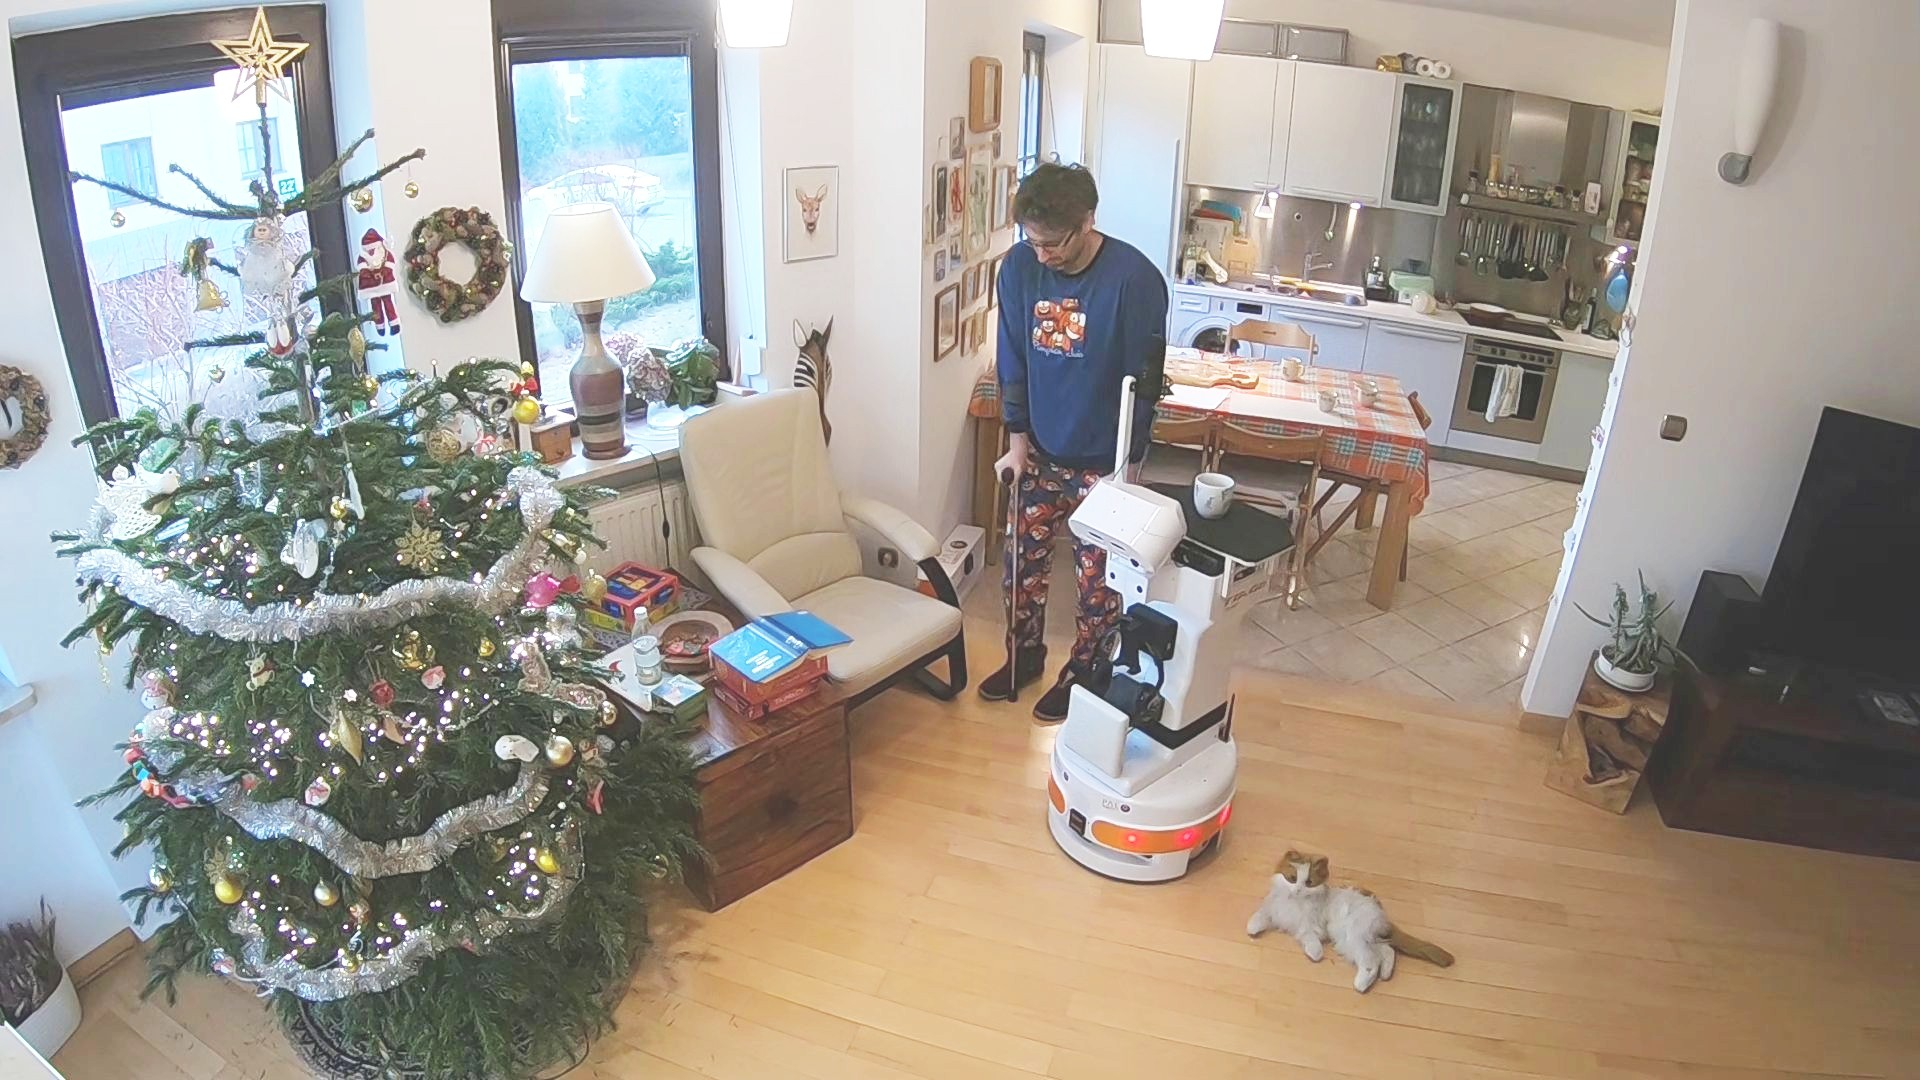
\includegraphics[width=0.9\columnwidth]{../imgs/herbatka_u_winiara.jpg}}
    \end{center}
    \caption{Transportation attendance by Rico robot \url{https://vimeo.com/670252925}}
    \label{fig:herbatka_u_winiara}
\end{figure}



The purpose of the following description is not to document the entire system but to illustrate, by example, representative aspects of the MeROS application.

\pagebreak

The part of the application scenario is conceptually presented in Fig.~\ref{fig:general_sd}.


\begin{figure}[H]
    \centering
    \begin{center}
    {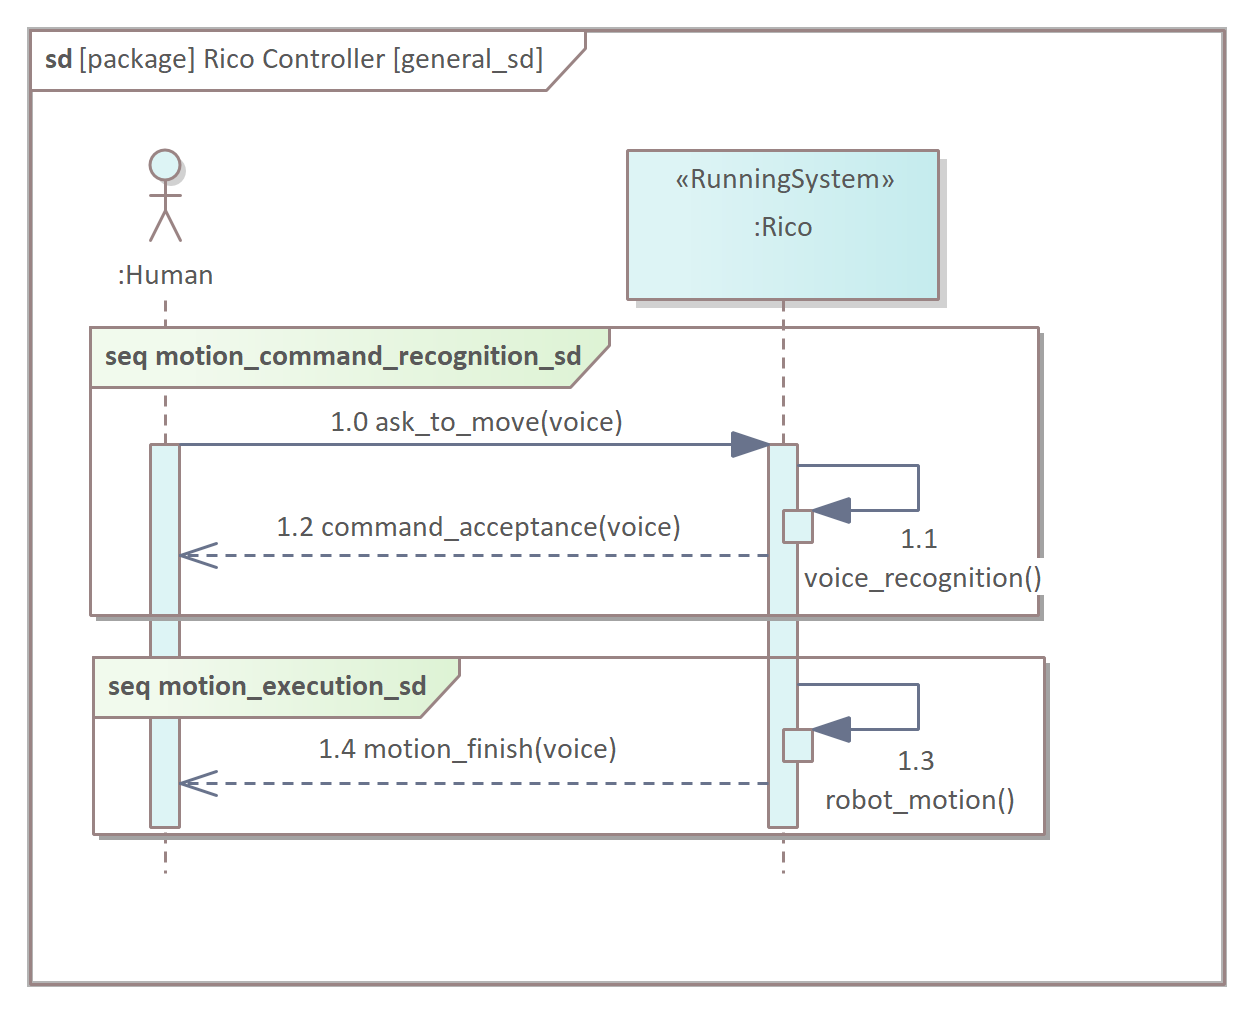
\includegraphics[scale=0.95]{../imgs/rico_pkg/general_sd.png}}
    \end{center}
    \caption{Concept scenario -- sd.}
    \label{fig:general_sd}
\end{figure}

Here, the system (<<RunningSystem>> \texttt{:Rico}) and its behaviour are formulated in a~general way. An actor (e.g. an elderly person) asks the robot to move. Then, the system recognises the voice command and vocally confirms the command's acceptance. Finally, the robot executes the motion and vocally informs that the motion is finished.
In the following part of the description, the <<RunningSystem>> \texttt{:Rico} and sequence diagram frame \texttt{motion execution} from Fig.~\ref{fig:general_sd} are presented in a explicit way.
The block definition diagram in Fig.~\ref{fig:rico_running_system_bdd} depicts the composition of <<RunningSystem>> \texttt{:Rico}.

\begin{figure}[H]
    \centering
    \begin{center}
    {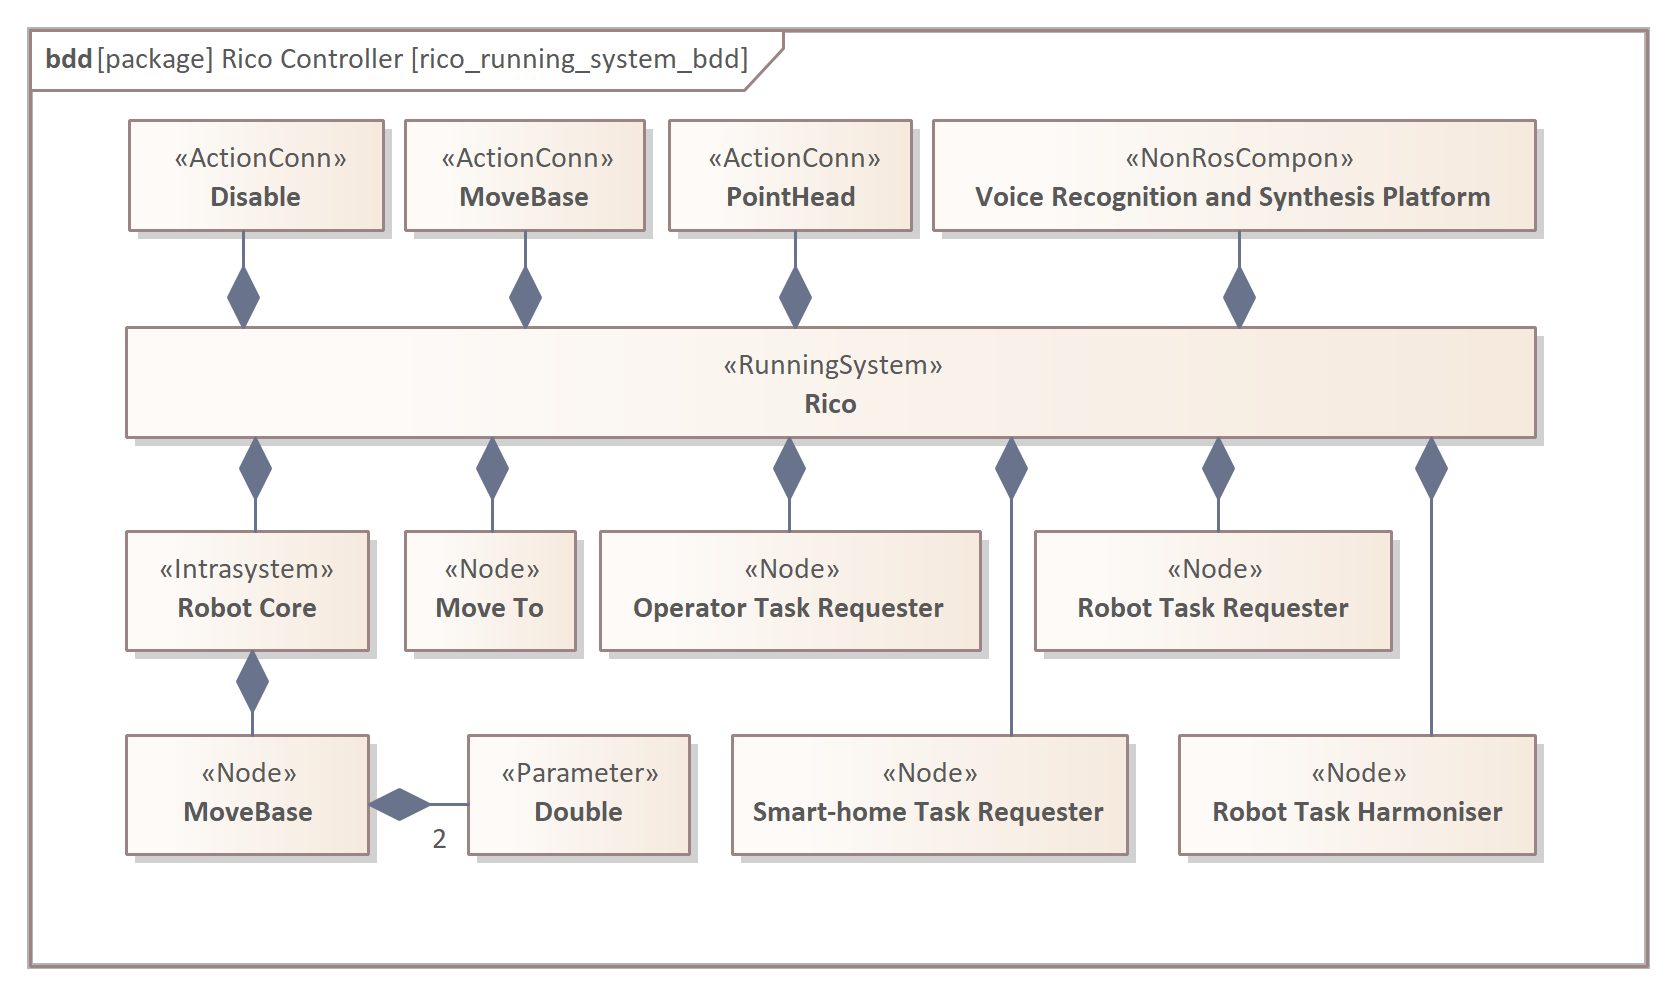
\includegraphics[scale=0.95]{../imgs/rico_pkg/rico_running_system_bdd.png}}
    \end{center}
    \caption{Rico <<RunningSystem>> composition -- bdd.}
    \label{fig:rico_running_system_bdd}
\end{figure}

The <<RunningSystem>> \texttt{:Rico} structure is depicted in Fig.~\ref{fig:rico_running_system_ibd}. Here, and in the following diagrams, the \texttt{rosout} and \texttt{ROS master} <<Node>>s were omitted to make the diagrams more compact. The specific label is needed for <<CommChannel>>, e.g., <<CommChannel>> \texttt{:Move To to Robot Core}, because this <<CommChannel>> is described later on.

\begin{figure}[H]
    \centering
    \begin{center}
    {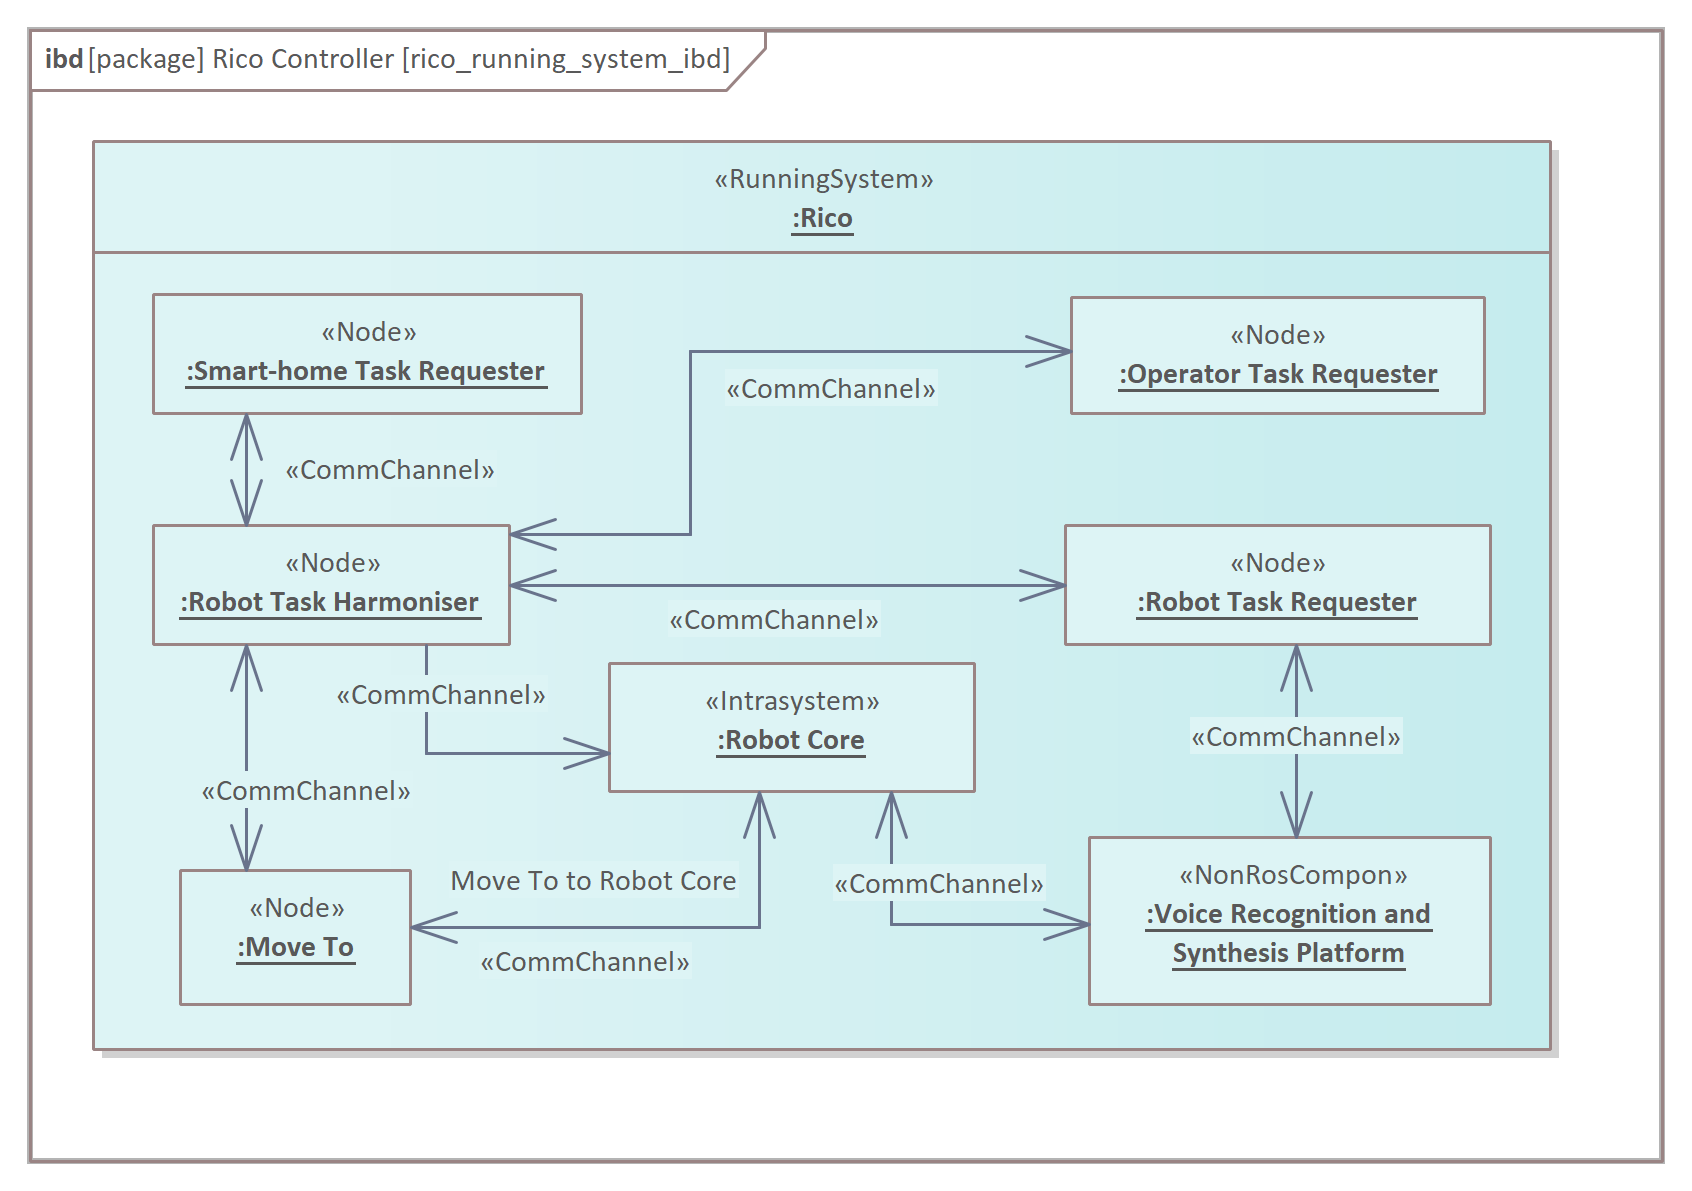
\includegraphics[scale=0.85]{../imgs/rico_pkg/rico_running_system_ibd.png}}
    \end{center}
    \caption{Structure of <<RunningSystem>> \texttt{:Rico} -- ibd.}
    \label{fig:rico_running_system_ibd}
\end{figure}

The system is based on TaskER framework \cite{tasker2020} developed from the RAPP approach to construct systems with variable structure \cite{zielinski2017variable}. The role of the TaskER is to schedule a robot’s tasks. It consists of (i) Task Requesters <<Node>>s to submit new tasks, (ii) Task Harmoniser <<Node>> to schedule tasks execution, (iii) dynamic <<Node>>s (here, <<Node>> \texttt{:Move To}) to execute a particular task on the robot hardware and (iv) cloud part, here <<NonRosCompon>> \texttt{:Voice Recognition and Synthesis Platform}. The common part of the controller is located in <<Intrasystem>> \texttt{:Rico}.

Fig.~\ref{fig:robot_core_ibd} illustrates how various instances of the same block are depicted in the model. Two <<Parameter>> Objects of the same classifier \texttt{:Double} are composed into <<Node>> \texttt{:MoveBase}.

\begin{figure}[H]
    \centering
    \begin{center}
    {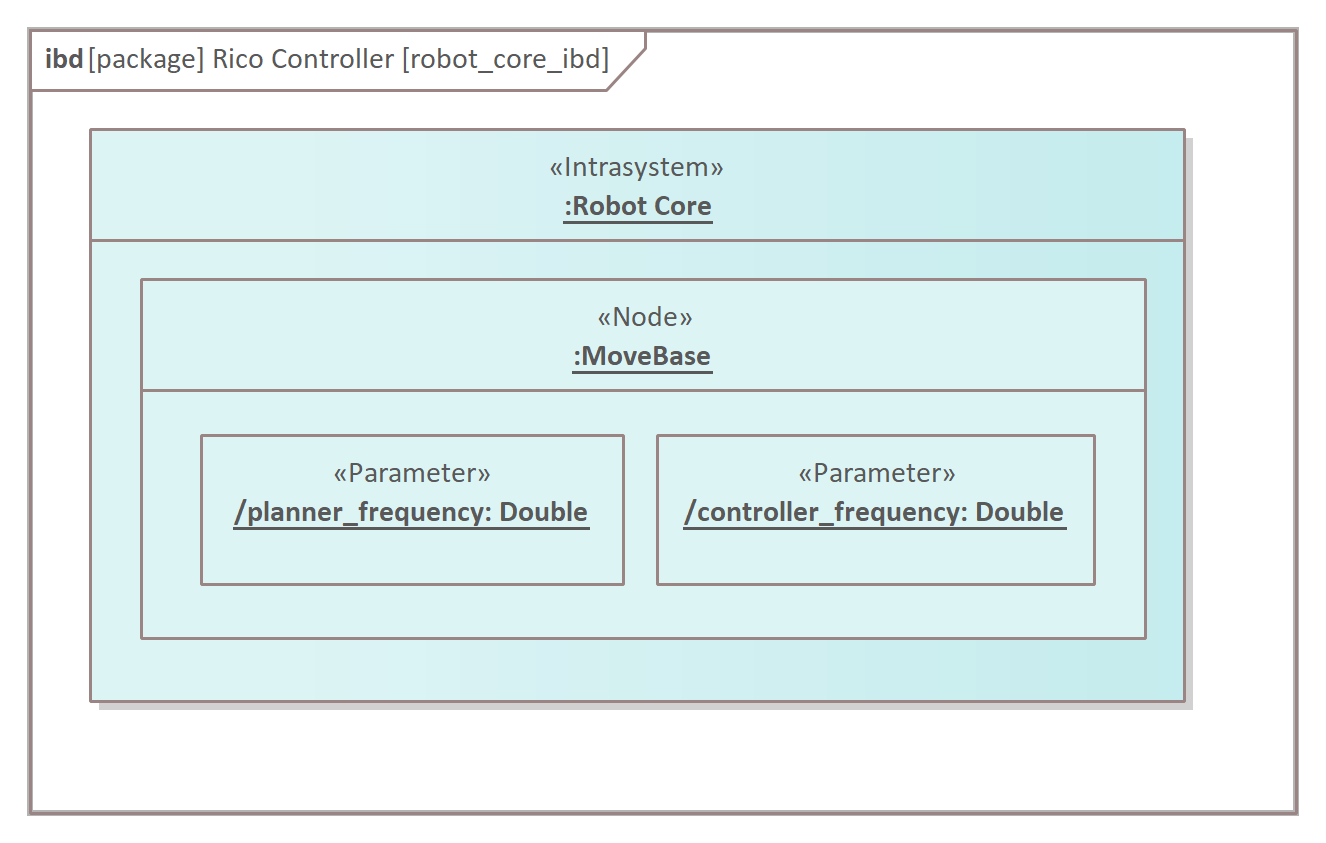
\includegraphics[scale=0.85]{../imgs/rico_pkg/robot_core_ibd.png}}
    \end{center}
    \caption{Selected elements of <<Intrasystem>> \texttt{:Robot Core} -- ibd.}
    \label{fig:robot_core_ibd}
\end{figure}


<<CommChannel>> \texttt{:Move To to Robot Core} is depicted in Fig.~\ref{fig:move_to_2_core_cm_ibd}. It comprises three actions.


\begin{figure}[H]
    \centering
    \begin{center}
    {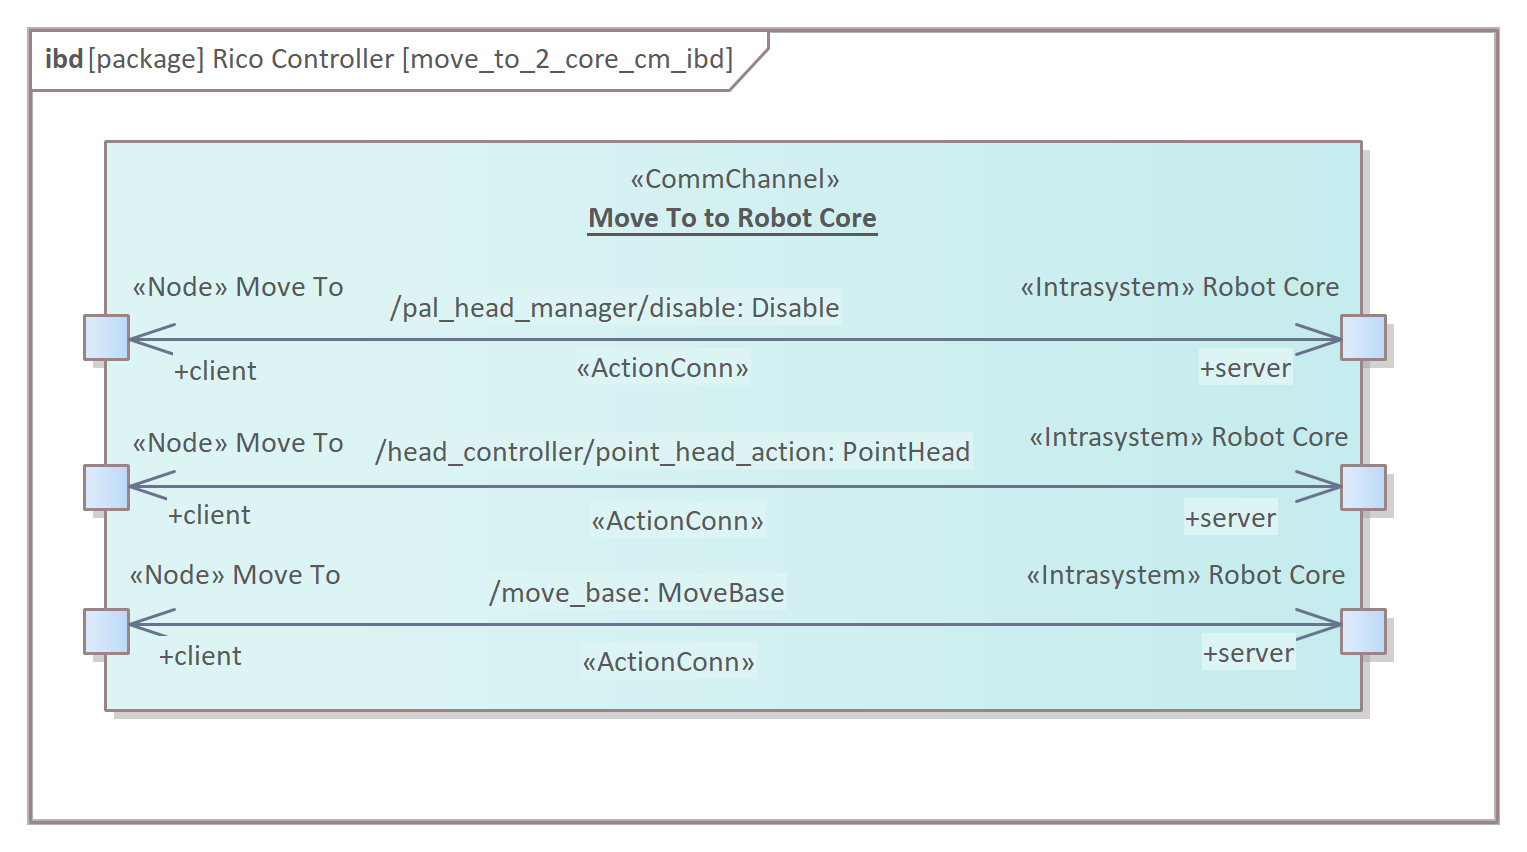
\includegraphics[scale=1.0]{../imgs/rico_pkg/move_to_2_core_cm_ibd.png}}
    \end{center}
    \caption{Example of <<CommChannel>> -- ibd.}
    \label{fig:move_to_2_core_cm_ibd}
\end{figure}


The part of the scenario generally described in Fig.~\ref{fig:general_sd} is depicted in detail in Fig.~\ref{fig:motion_execution_sd}. The presentation remains conceptual from the behavioural point of view, but it considers the particular parts of the <<RunningSystem>> \texttt{:Rico}.

\begin{figure}[H]
    \centering
    \begin{center}
    {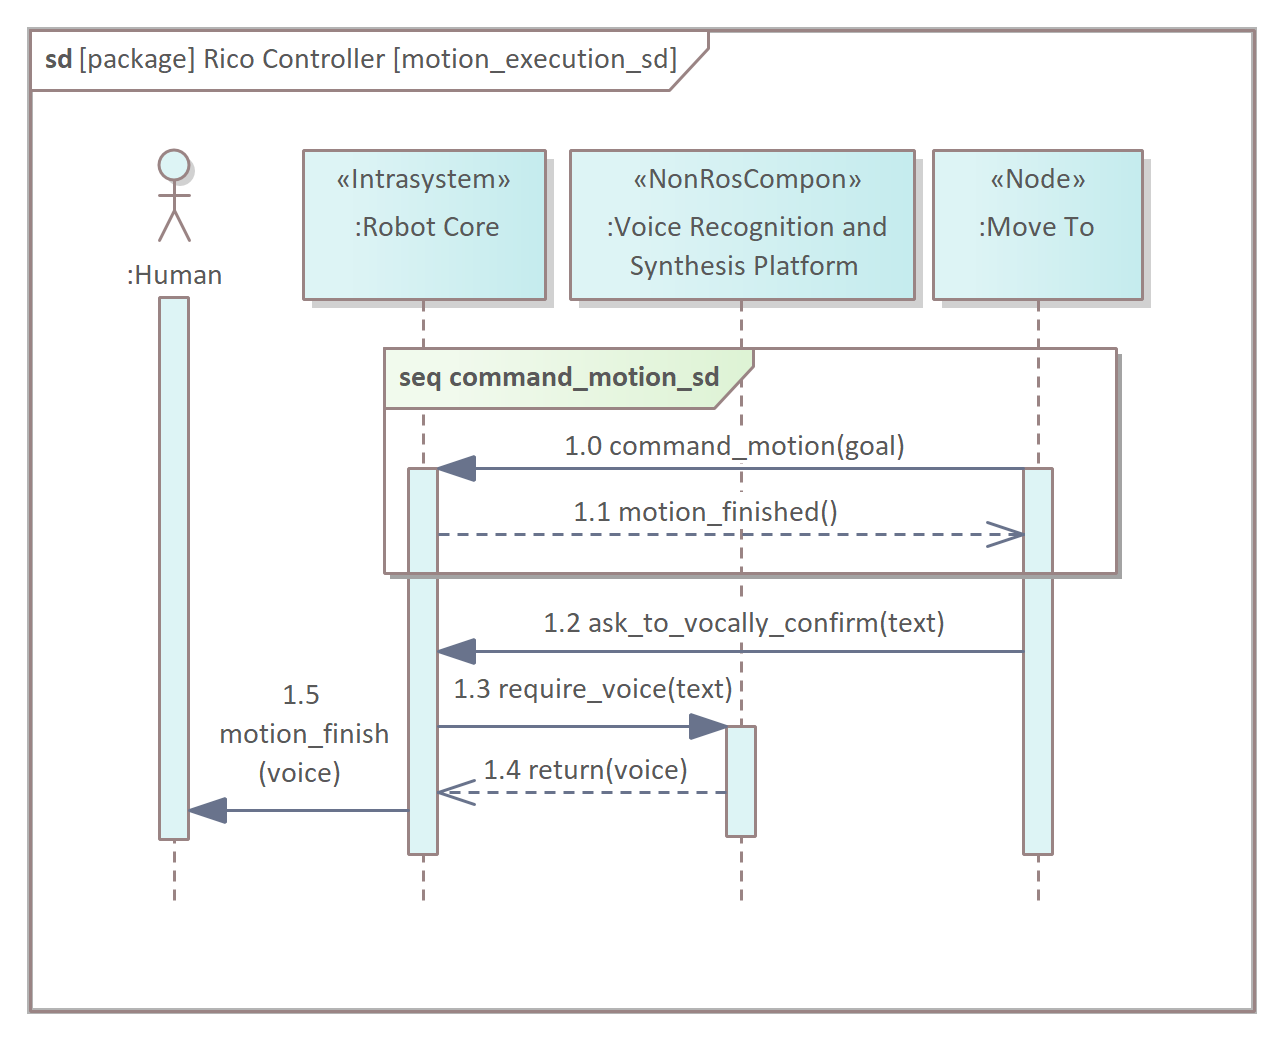
\includegraphics[scale=1.1]{../imgs/rico_pkg/motion_execution_sd.png}}
    \end{center}
    \caption{Motion execution operation -- sd.}
    \label{fig:motion_execution_sd}
\end{figure}

\pagebreak


Finally, the particular communication methods are specified on the most detailed, ROS-specific level (Fig.~\ref{fig:command_motion_sd}). The command\_motion operation includes the sequence of four steps of communication. Three Actions realise the communication, one utilised twice. The diagram comprises extra notes that make it easier to interpret.

\begin{figure}[H]
    \centering
    \begin{center}
    {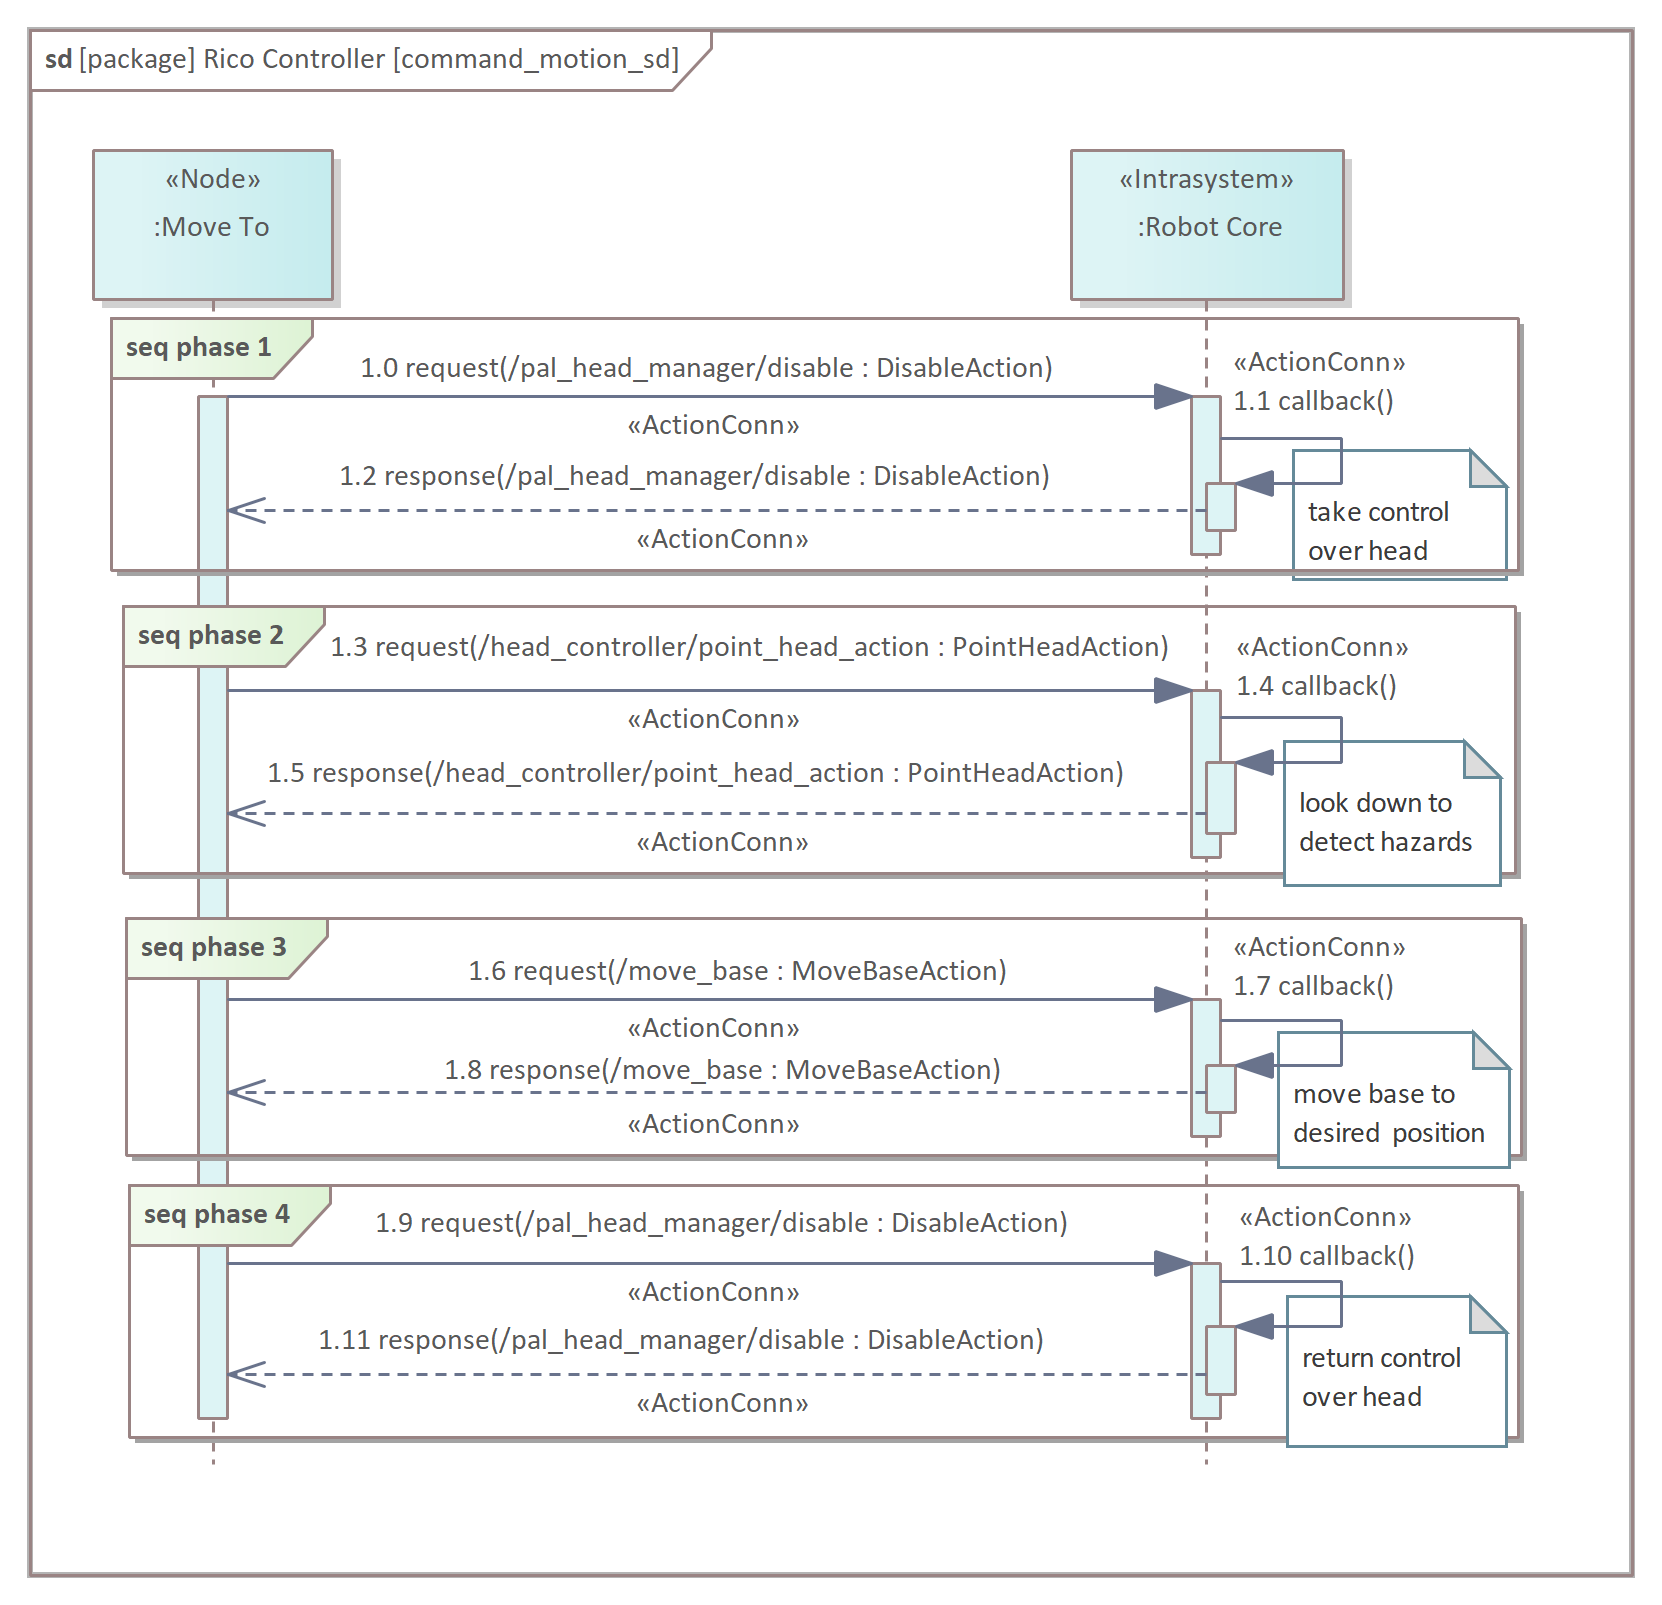
\includegraphics[scale=1.1]{../imgs/rico_pkg/command_motion_sd.png}}
    \end{center}
    \caption{Command motion operation with detailed Communication methods presentation -- sd.}
    \label{fig:command_motion_sd}
\end{figure}

\pagebreak

The part of the <<Workspace>> \texttt{:Rico} that includes previously mentioned elements is presented in Fig.~\ref{fig:rico_workspace_nodes_bdd} and Fig.~\ref{fig:rico_workspace_msgs_bdd}.

\begin{figure}[H]
    \centering
    \begin{center}
    {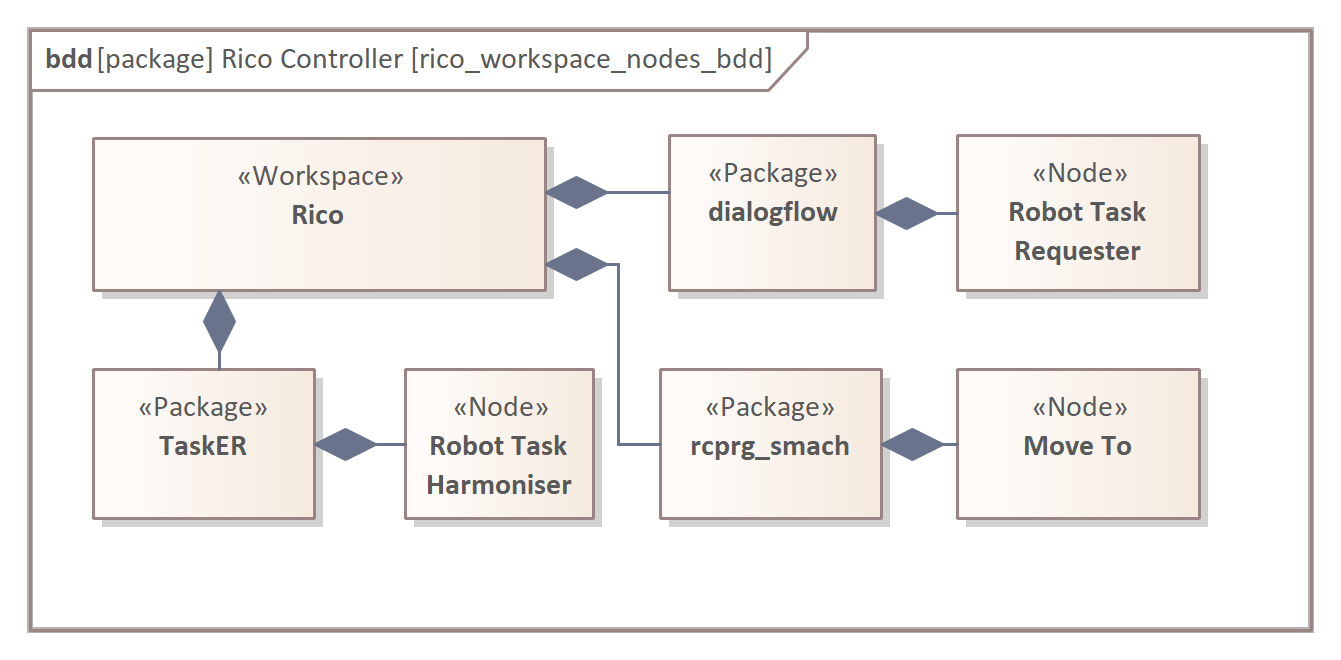
\includegraphics[scale=1.0]{../imgs/rico_pkg/rico_workspace_nodes_bdd.png}}
    \end{center}
    \caption{Rico <<Workspace>> composition -- Packages with Nodes -- bdd.}
    \label{fig:rico_workspace_nodes_bdd}
\end{figure}

\begin{figure}[H]
    \centering
    \begin{center}
    {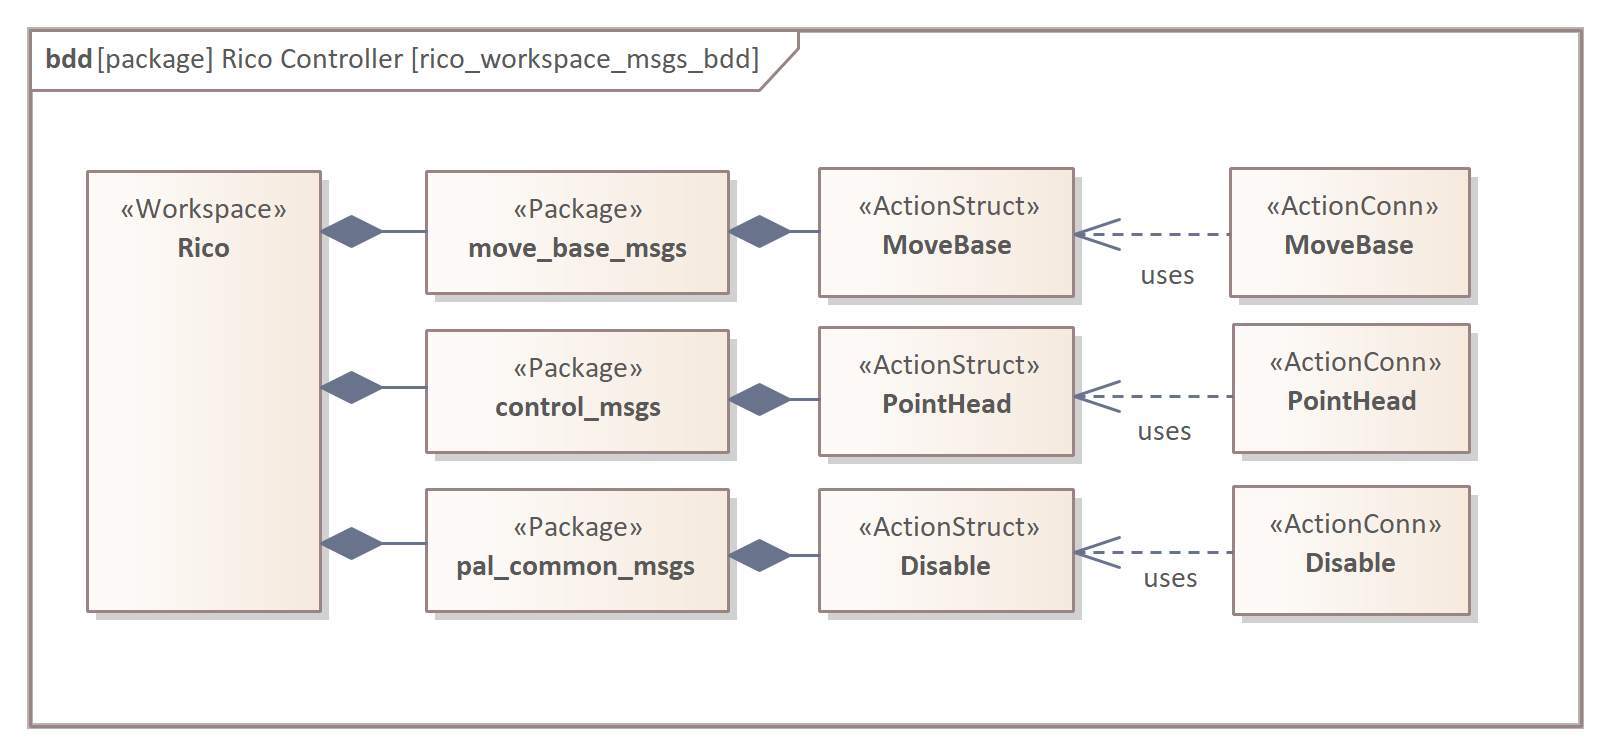
\includegraphics[scale=1.0]{../imgs/rico_pkg/rico_workspace_msgs_bdd.png}}
    \end{center}
    \caption{Rico <<Workspace>> composition -- Packages with Msgs -- bdd.}
    \label{fig:rico_workspace_msgs_bdd}
\end{figure}

